\documentclass[tikz]{standalone}
%\usetikzlibrary{positioning}
\usetikzlibrary{decorations.pathmorphing}
\usetikzlibrary{decorations.markings}
\usetikzlibrary{shapes.misc}
\usetikzlibrary{intersections}
\usetikzlibrary{arrows}
\tikzset{>={latex}}
\tikzstyle{X}=[cross out, draw, orange, scale = 0.75, thick]

\begin{document}
	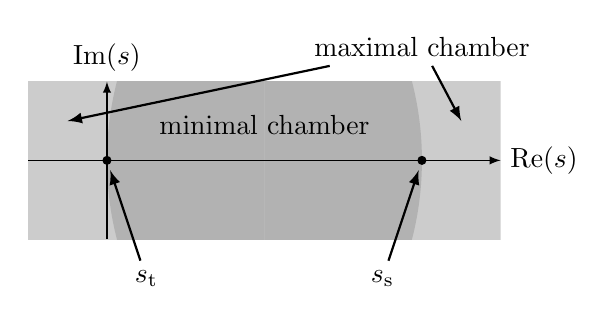
\begin{tikzpicture}[scale=2]
		\begin{scope}
			\clip (-.5, -.5) rectangle (2.5, .5);
			\fill[black!20] (1, 0) circle (3);
			%\fill[black!30] (1, 0) circle (1);		
		\end{scope}
		
		\begin{scope}
			\clip (-.5, -.5) rectangle (1, .5);		
			\fill[black!30] (2, 0) circle (2);
		\end{scope}

		\begin{scope}
			\clip (1, -.5) rectangle (2.5, .5);		
			\fill[black!30] (0, 0) circle (2);
		\end{scope}

		
		\draw[->] (-.5, 0) -- (2.5, 0);
		\node[right] at (2.5, 0) {Re$(s)$};
		\draw[->] (0, -0.5) -- (0, .5);
		\node[above] at (0, 0.5) {Im$(s)$};
		
		\draw[fill] (0,0) circle (.025);
		\node (s_t) at (0,0) {};
		\node (s_t_label) at (.25, -.75) {$s_\mathrm{t}$};
		\draw[->, thick] (s_t_label) -- (s_t); 

	
		\draw[fill] (2,0) circle (.025);
		\node (s_s) at (2,0) {};
		\node (s_s_label) at (2 - .25, -.75) {$s_\mathrm{s}$};
		\draw[->, thick] (s_s_label) -- (s_s); 
		
		\node[above] (region_1_label) at (2, .6) {maximal chamber};
		\draw[->, thick] (region_1_label) -- (-.25,.25); 
		\draw[->, thick] (region_1_label) -- (2.25,.25);
				
		\node[above] (region_2_label) at (1, 0.1) {minimal chamber};
		
	\end{tikzpicture}

\end{document}